%!TeX spellcheck = en-US

%\chapter{Handling the Noise of the Web-Genres}
\chapter{Experimental Analysis of Open-set WGI Methods}

\label{chap:noise}

%----------------------------------------------------------------------------------------

% Define some commands to keep the formatting separated from the content
\newcommand{\keyword}[1]{\textbf{#1}}
\newcommand{\tabhead}[1]{\textbf{#1}}
\newcommand{\code}[1]{\texttt{#1}}
\newcommand{\file}[1]{\texttt{\bfseries#1}}
\newcommand{\option}[1]{\texttt{\itshape#1}}

%----------------------------------------------------------------------------------------

\section{Introduction}\label{chap:noise:sec:intro}

Based on the evaluation framework described in the previous chapter, it is now possible to evaluate the open-set WGI algorithms presented in chapter \ref{chap:openset}. Certainly, any kind of empirical evaluation depends on the dataset that is used for estimating the performance of the examined models. Each dataset has its weaknesses and this might lead to an over-estimation or under-estimation of performance of the examined methods in more realistic conditions. However, what we want to study here is the comparison of performance of different approaches on exactly the same datasets and experimental setup to extract conclusions about the relative improvement in performance of one method with respect to another.

In this thesis, we focus on the effect of noise in open-set WGI approaches. In particular, we want to examine the performance of WGI methods when either unstructured or structured noise is available. The former is a realistic scenario in most WGI applications where it is difficult, if not impossible, to define the genre of a large part of the web. In such cases, it is better to assume that the unknown class comprises any kind of web-pages that do not belong to the known genres. On the other hand, this makes the definition of noise chaotic and extremely heterogeneous. 

The case of structured noise offers the opportunity to study the performance of open-set WGI methods when the heterogeneity of noise can be controlled. The assumption that information about the unknown classes is available (although the classifier has no training examples for these classes) is not unrealistic. For example, an open-set WGI system that aims to recognize news articles should not be distracted by blogs. That is, we know that blogs exist and perhaps comprise the majority of noise in that system but we do not provide training examples for that class.

Among the three open-set WGI methods proposed in this thesis, OCSVM and RFSE are examined in this Chapter while NNDR is thoroughly tested in Chapter \ref{chap:word_embeddings}. The reason for this is that NNDR is especially difficult to be tested in conditions of structured noise, especially when limited known classes are available since a part of known classes have to be used for estimating the open space risk. Therefore, NNDR is only tested with unstructured noise.

The estimation of performance of WGI methods also depends on the applications they are going to be used. Some applications require high precision (e.g., ranking genre-based search results). On the other hand, it is rather unusual to aim for high recall with the cost of reducing precision in WGI-related applications. The experimental analysis should also reflect these facts.

Another crucial issue is the representation of web-pages. As already explained in chapter \ref{chap:openset} the dimensionality of representation, the existence of irrelevant and redundant features can severely harm the performance of certain open-set WGI methods. Therefore, it is important to study how different text representation schemes, especially the ones that were found to be the more reliable ones in previous WGI studies, affect the performance of the examined methods. 

In the remaining of this chapter, we first describe the datasets used in this study and the experimental setup. Then, we present the experimetntal results in open-set WGI when either unstructured noise or structured noise is available. Finally, we summarize the drawn conclusions.

\section{Corpora}\label{chap:noise:sec:corpora}
In this paper we study the performance of the open-set classification models on the WGI task. In particular, the two open-set algorithms described above are analytically tested on benchmark corpora. In particular, our experiments are based on the following corpora already used in previous work in WGI \parencite{meyer2004genre,santini2007automatic,kanaris2009learning}:

\begin{enumerate}
	\item \textit{SANTINIS} \parencite{mehler2010genres_on_web}: This is a corpus comprising 1,400 English web pages evenly distributed into 7 genres as well as 80 BBC web pages evenly categorized into 4 additional genres. In addition, it comprises a random selection of 1,000 English web pages taken from the SPIRIT corpus \parencite{joho2004spirit}. The latter can be viewed as noise in this corpus. Details are given in table \ref{chap:noise:tbl:genre_tags}.
	\item \textit{KI-04} \parencite{meyer2004genre}: This is a collection of 1,205 English web pages unevenly categorized into 8 genres. Details can be seen in table \ref{chap:noise:tbl:genre_tags}.
\end{enumerate}


\section{Experimental Setup}\label{chap:noise:sec:experimental_setup}

The text representation features used in this thesis are based exclusively on textual information from web pages excluding any structural information, URLs, etc. This does not mean that we consider other kinds of information (e.g., HTML-based features, URL-based features etc.) as less important in WGI. However, information coming from the text itself is less likely to be affected by technology-related choices that can be easily altered through time. By focusing on the text of the web pages we ensure that the drawn conclusions are more reliable and long lasting.

Based on the good results reported in \parencite{sharoff2010web,kanaris2009learning,Asheghi2015} as well as some preliminary experiments, the following document representation schemes are examined: 

\begin{itemize}
    \item Character 4-grams (C4G)
    \item Word unigrams (W1G)
    \item Word 3-grams (W3G)
    \item Part-of-speech 3-grams (POS3G)
\end{itemize}

The Stanford POS tagger has been used for POS3G creation. We use the Term-Frequency (TF) weighting scheme and the feature space is defined by a \textit{Vocabulary} which is extracted based on the terms appearing at training set only. There is no pre-processing of textual data (e.g., stop word removal, stemming etc.) since in style-based text categorization tasks these processes remove significant stylistic information \parencite{stamatatos2009survey}.

Each open-set WGI method has some hyper-parameters to be tuned. In order to extract the best possible parameter settings for each classification method we apply grid-search over the space of all parameter value combinations. This is not the most sophisticated approach but ensures that the extracted parameter values will fine-tune the model for the specific dataset.

As concerns OCSVM method, two parameters have to be tuned: the number of features $F$ and $\nu$. For the former, we used $F=$\{1k, 5k, 10k, 50k, 90k\}, of most frequent terms of the vocabulary. Following the reports of previous studies \parencite{scholkopf1999estimating} and some preliminary experiments, we examined $\nu$=\{0.05, 0.07, 0.1, 0.15, 0.17, 0.3, 0.5, 0.7, 0.9\}. In comparison to \parencite{pritsos2013open}, this set of parameter values is more extended. 

With respect to RFSE, four parameters should be set: the vocabulary size $F$, the number of features used in each iteration $fs$, the number of iterations \textit{I}, and the threshold $\sigma$. We examined $F$=\{5k, 10k, 50k, 100k\}, $fs$=\{1k, 5k, 10k, 50k, 90k\}, \textit{I}=\{10, 50, 100\} (following the suggestion in \parencite{koppel2011authorship} that more than 100 iterations does not improve significantly the results) and $\sigma$\textit{=\{0.5, 0.7, 0.9\}} (based on some preliminary tests). Additionally, in this thesis we test three document similarity measures used in RFSE approach: cosine similarity, MinMax similarity, and Combo (as defined in Section \ref{chap:openset:sec:RFSE_Description}). 

%Finally, for the NNDR approach, there are two parameters to be tuned: $lambda$ and DRT. The considered values are: $\lambda =\{0.2, 0.5, 0.7\}$, $DRT=\{0.4, 0.6, 0.8, 0.9\}$. 

%\textcolor{red}{WHAT ABOUT $P_1$ and $P_2$ (in the estimation of DRT)}

\begin{table}[t]
\center
\begin{tabular}{|l|l|l|l|}
\hline
\multicolumn{2}{|c|}{SANTINIS} & \multicolumn{2}{c|}{KI-04}\tabularnewline
\hline
\multicolumn{1}{|c|}{Genre} & \multicolumn{1}{c|}{Pages} & \multicolumn{1}{c|}{Genre} & \multicolumn{1}{c|}{Pages}\tabularnewline
\hline
\multicolumn{1}{|l|}{Blog} & \multicolumn{1}{c|}{200} & \multicolumn{1}{l|}{Article} & \multicolumn{1}{c|}{127}\tabularnewline
\multicolumn{1}{|l|}{Eshop} & \multicolumn{1}{c|}{200} & \multicolumn{1}{l|}{Discussion} & \multicolumn{1}{c|}{127}\tabularnewline
\multicolumn{1}{|l|}{FAQ} & \multicolumn{1}{c|}{200} & \multicolumn{1}{l|}{Download} & \multicolumn{1}{c|}{152}\tabularnewline
\multicolumn{1}{|l|}{Frontpage} & \multicolumn{1}{c|}{200} & \multicolumn{1}{l|}{Help} & \multicolumn{1}{c|}{140}\tabularnewline
\multicolumn{1}{|l|}{Listing} & \multicolumn{1}{c|}{200} & \multicolumn{1}{l|}{Link Collection} & \multicolumn{1}{c|}{208}\tabularnewline
\multicolumn{1}{|l|}{Personal Home Page} & \multicolumn{1}{c|}{200} & \multicolumn{1}{l|}{Portrayal-Non Private} & \multicolumn{1}{c|}{179}\tabularnewline
\multicolumn{1}{|l|}{Search Page} & \multicolumn{1}{c|}{200} & \multicolumn{1}{l|}{Portrayal- Private} & \multicolumn{1}{c|}{131}\tabularnewline
\multicolumn{1}{|l|}{DIY Mini Guide (BBC)} & \multicolumn{1}{c|}{20} & \multicolumn{1}{l|}{Shop} & \multicolumn{1}{c|}{175}\tabularnewline
\multicolumn{1}{|l|}{Editorial (BBC)} & \multicolumn{1}{c|}{20} &  & \tabularnewline
\multicolumn{1}{|l|}{Features (BBC)} & \multicolumn{1}{c|}{20} &  & \tabularnewline
\multicolumn{1}{|l|}{Short Bio (BBC)} & \multicolumn{1}{c|}{20} &  & \tabularnewline
\multicolumn{1}{|l|}{Noise (Spirit1000)} & \multicolumn{1}{c|}{1000} &  & \tabularnewline
\hline
\end{tabular}
\caption {Corpora descriptions and amount of pages per genre.}
\label{chap:noise:tbl:genre_tags}
\end{table}


\section{WGI with Unstructured Noise}\label{chap:noise:sec:WGI_noise}

The two open-set algorithms RFSE and OCSVME, describe in sections \ref{chap:openset:sec:alg:OCSVM_Ensemble} and \ref{chap:openset:sec:alg:RFS-Ensemble}, are initially tested on SANTINIS corpus which as explained above is an Unstructured Noise, samples corpus.   

In the training phase, only the 11 known genres are considered. In the testing phase, the noise pages coming from the SPIRIT corpus are also used. It is important to be noted that information about the true genre of these pages is not available. The 10-fold cross validation is performed where in each fold the full set of 1,000 pages of noise is included. This evaluation strategy is giving a more realistic evaluation framework since the size of the noise is much greater than the size of any genre included in the given palette.

Figures \ref{chap:noise:fig:MacroPRC_OCSVME_W3G_W1G_C4G_OPTIMAL_SANTINIS} and \ref{chap:noise:fig:MacroPRC_RFSE_W3G_W1G_C4G_OPTIMAL_SANTINIS} depict the Precision-Recall curves (PRC) of OCSVM and RFSE models, respectively. For each model and each one of the three document representations, the parameters that maximize performance with respect to the $F_{1}$-measure are used. Remember from section \ref{chap:eval_methods:sec:roc_prc} whenever recall does not reach 1.0 this means that some pages belonging to known classes were classified as unknown. 

In all cases, RFSE outperforms OCSVM. Moreover, for both methods, W3G seems to be the best feature type for this corpus, followed by C4G. OCSVM performance is only comparable with RFSE when W3G is used.

\hfill \break


\begin{figure}[t]
	\begin{center}
    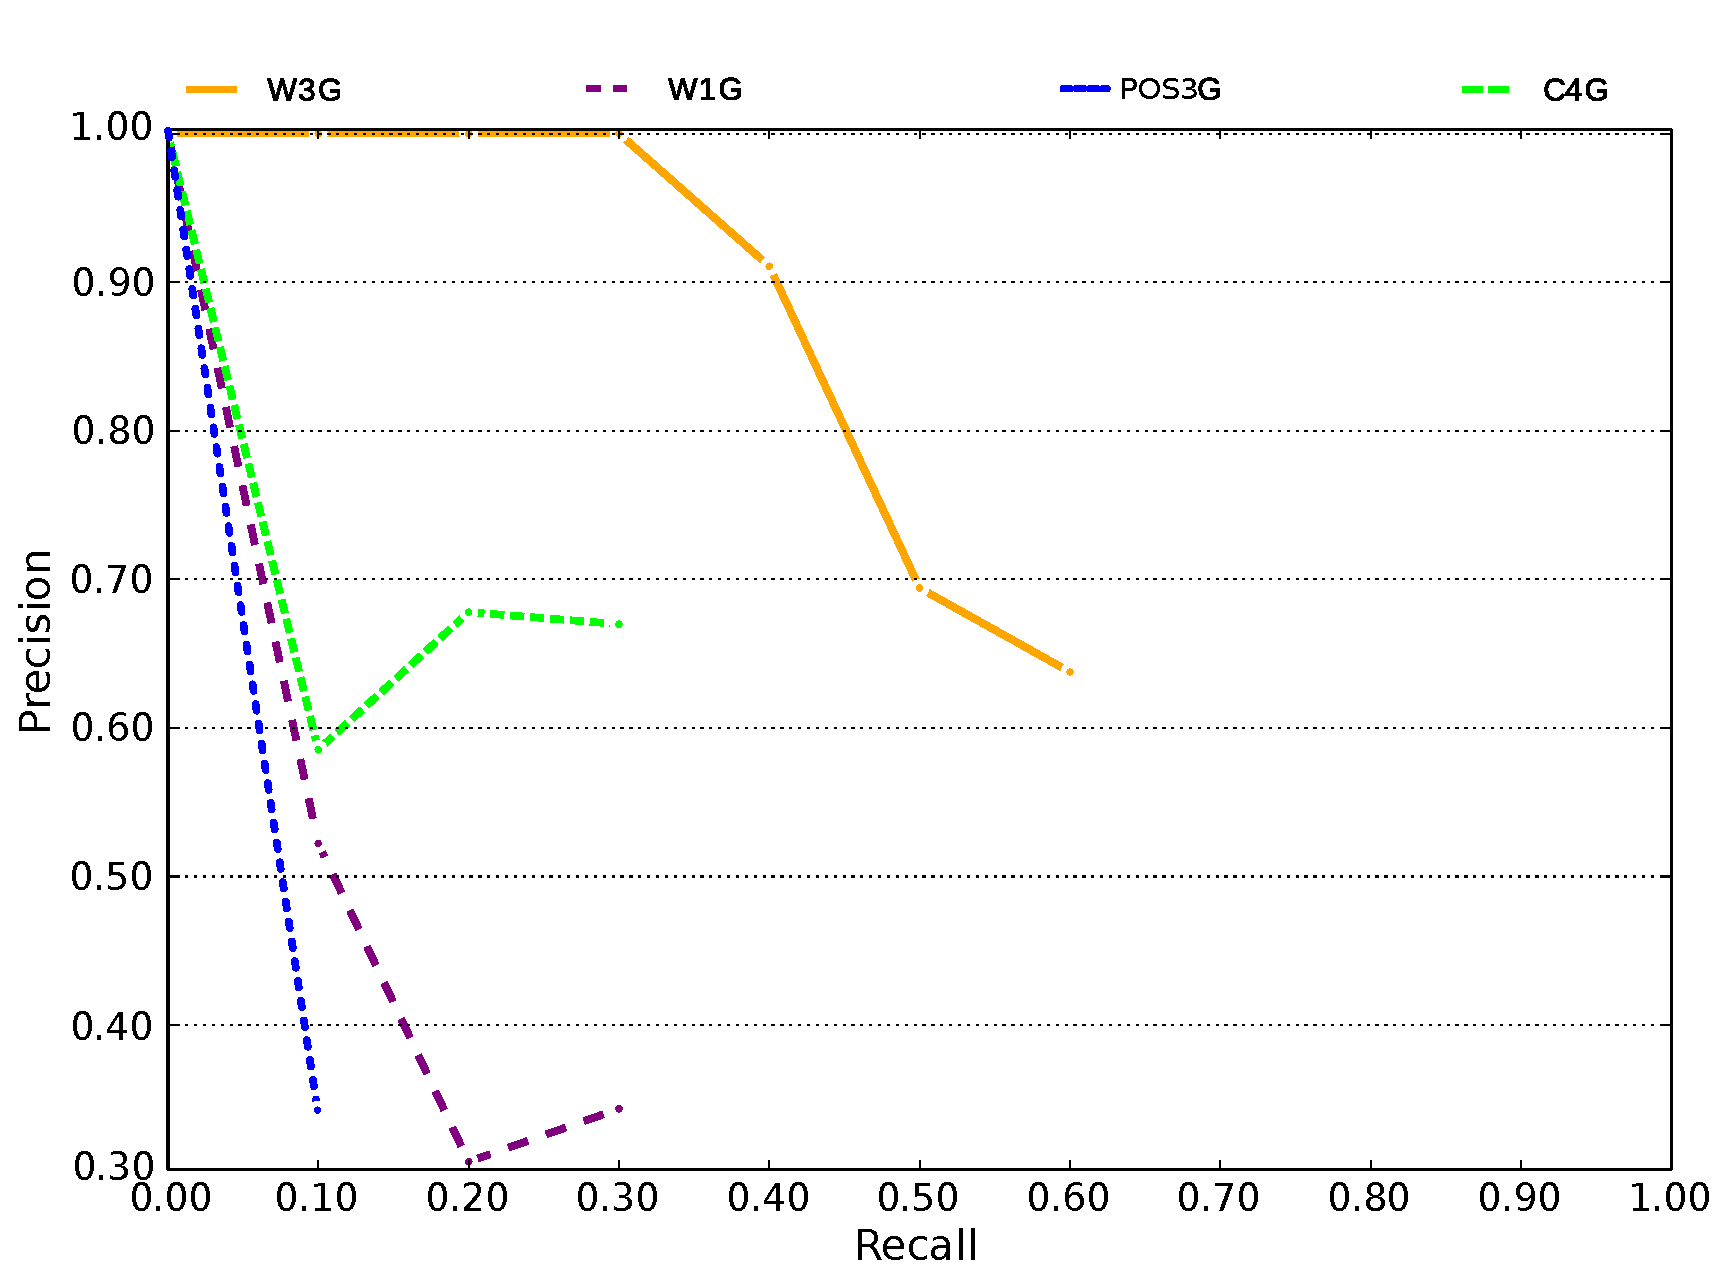
\includegraphics[scale=0.45]{Figures/OCSME_Best_per_DocRep.eps}
	\caption{Precision-Recall Curves of OCSVM models on SANTINIS corpus using W1G, W3G, and C4G features.}
	\label{chap:noise:fig:MacroPRC_OCSVME_W3G_W1G_C4G_OPTIMAL_SANTINIS}
	\end{center}
\end{figure}

\begin{figure}[t]
	\begin{center}
    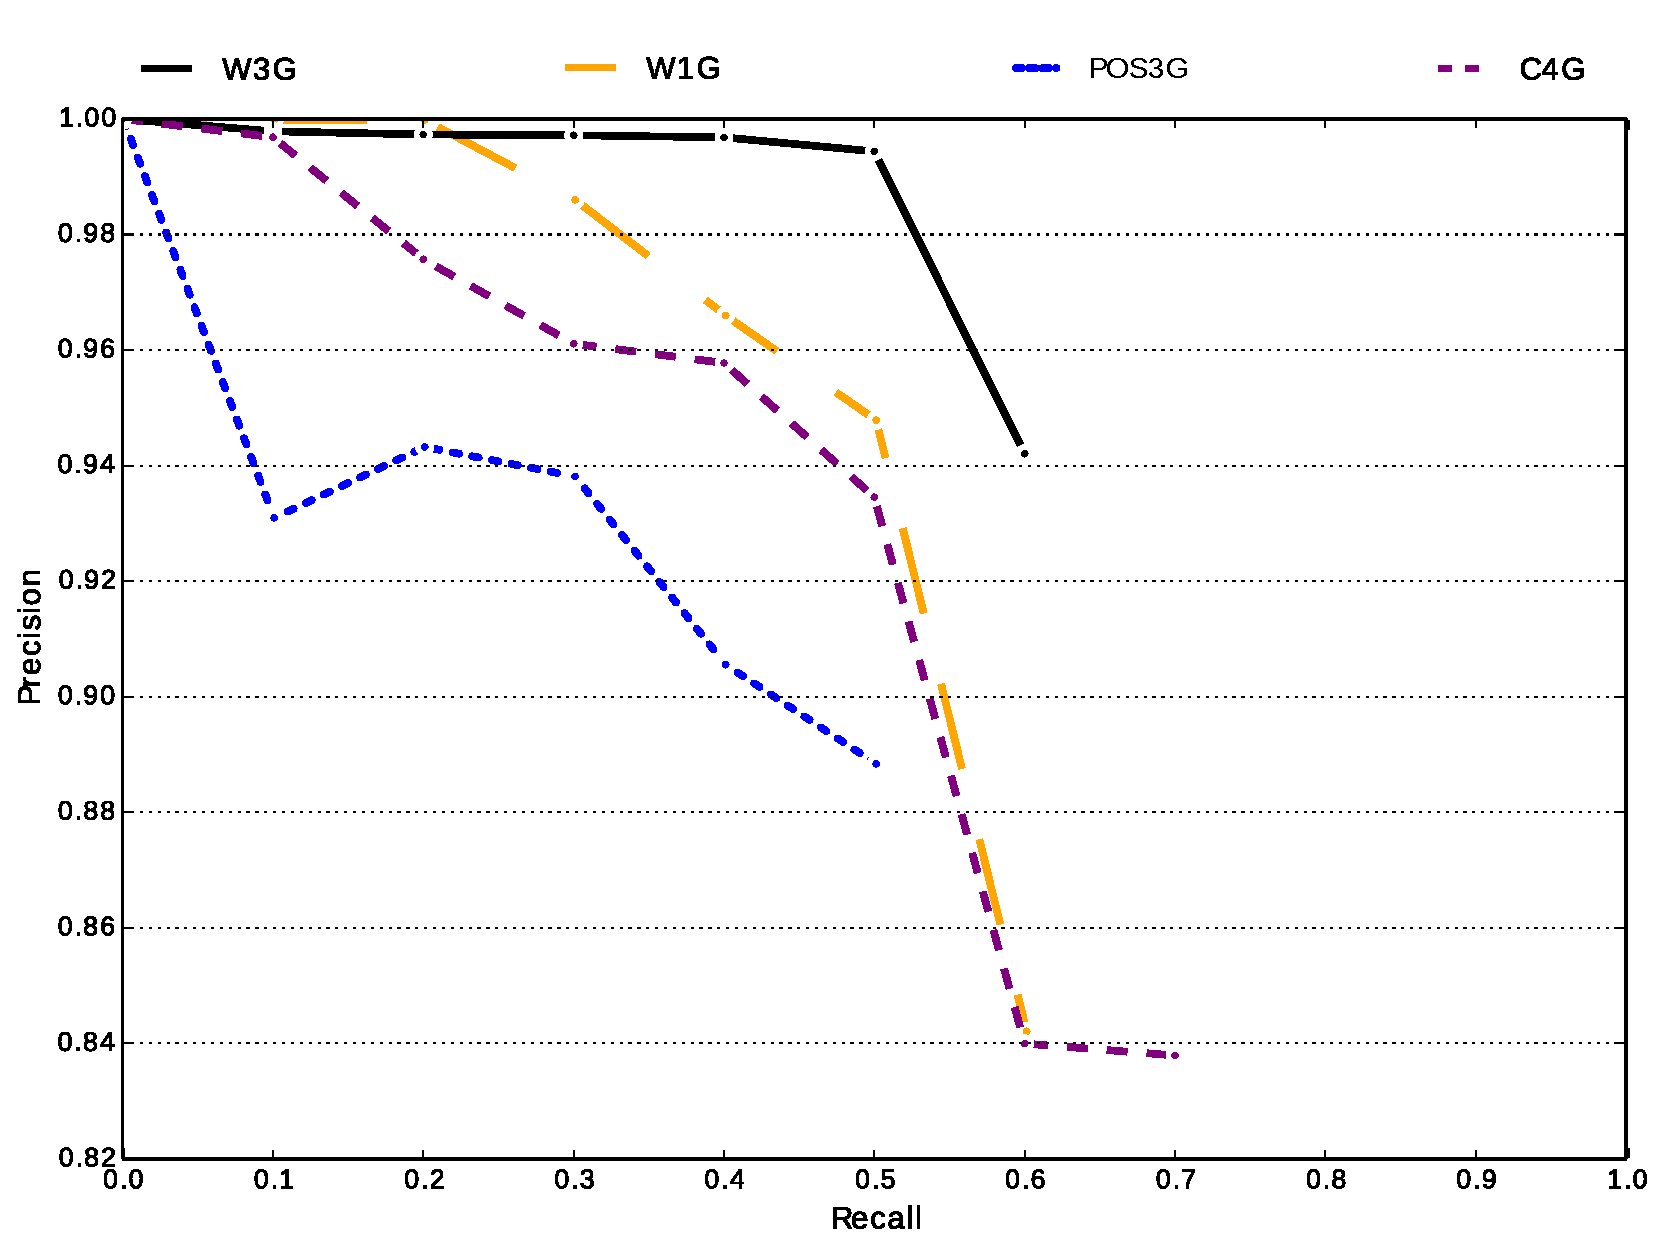
\includegraphics[scale=0.45]{Figures/RFSE_Best_per_DocRep.eps}
	\caption{Precision-Recall Curves of RFSE models on SANTINIS corpus using W1G, W3G, and C4G features.}
	\label{chap:noise:fig:MacroPRC_RFSE_W3G_W1G_C4G_OPTIMAL_SANTINIS}
	\end{center}
\end{figure}

The performance of the open-set WGI methods are further explored by selecting parameter settings with different optimization criteria. Tables \ref{chap:noise:tbl:OCSVME_SANTINIS} and \ref{chap:noise:tbl:RFSE_SANTINIS} show the combination of parameters that optimize performance of OCSVM and RFSE based on AUC, $F_{1}$ and $F_{0.5}$. 

In the tables \ref{chap:noise:tbl:OCSVME_SANTINIS} and \ref{chap:noise:tbl:RFSE_SANTINIS} the values are presented, of all three performance measures where, for every row, one of them is maximized. It is clear that the performance in all cases is maximized when W3G document representation is used. In previous studies based on a closed-set framework, C4G was the document type of features to maximize performance \parencite{Sharroff2010}. This indicates that contextual and content information is important for this corpus \parencite{Asheghi2015}.

In addition, in almost all cases, RFSE models are far more effective than OCSVM. Another important conclusion is that the optimization criterion plays a crucial role for the properties of the model especially for RFSE. When AUC is maximized, recall is favored. On the other hand, while $F_{1}$ is maximized, precision is substantially increased. Fig. \ref{chap:noise:fig:MacroPRC_RFSE_OCSVME_SANTINIS} shows the performance of OCSVM and RFSE models when AUC and $F_{1}$ criteria are used to select parameter settings. As can be seen, the RFSE model based on $F_{1}$ maximization avoids to make wrong decisions and leaves a large number of web pages unclassified. On the other hand, the model optimized by AUC prefers to make a lot of errors in order to recognize more web pages of known genres. OCSVM models seem not significantly affected. Note that choosing between WGI models that prefers precision over recall and vice versa is an application-specific task.



\begin{figure}[t]
\begin{center}
    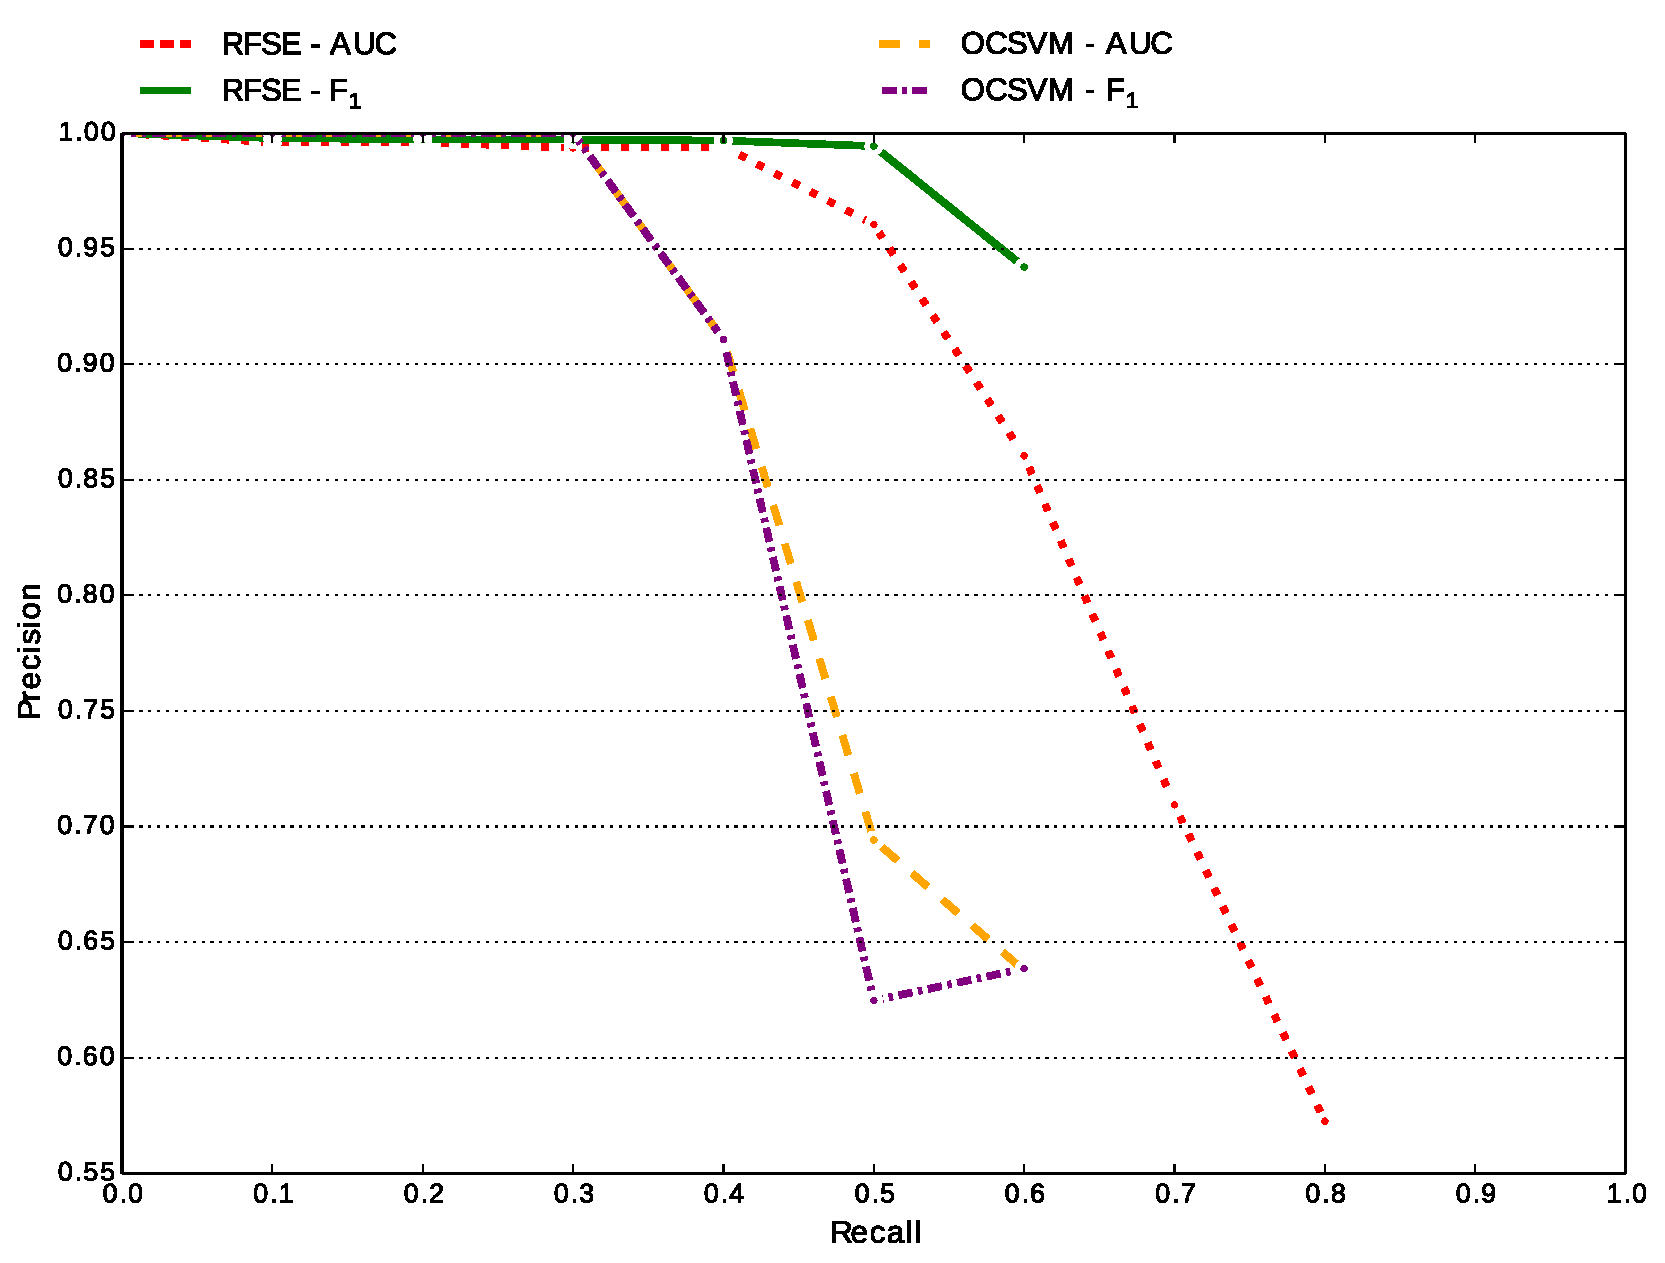
\includegraphics[scale=0.45]{Figures/MacroPRC11AVG_RFSE_OCSVME_SANTINIS_2.eps}
	\caption{Precision-Recall Curves of OCSVM and RFSE models on SANTINIS corpus optimized either by AUC or $F_{1}$.}
	\label{chap:noise:fig:MacroPRC_RFSE_OCSVME_SANTINIS}
	\end{center}
\end{figure}

% 7Genres
%
\begin{table}[t]
\centering




\pgfplotstableset{
    create on use/Criterion/.style={ create col/set list={AUC, $F_{1}$, $F_{0.5}$} },
	columns/DocRep/.style={string type},
	create on use/DocRep/.style={ create col/set list={W3G, W3G, W3G} },
	columns/DocRep/.style={string type}
}

\pgfplotstabletypeset[
		fixed,
		precision=3,
		col sep=comma,
		every head row/.style={
			before row = \toprule,
			after row=\midrule,
		},
		every last row/.style={after row=\bottomrule \\},
		columns={Criterion, DocRep, 0, 1, 2, 3, 4, 5, 6, 7},
		columns/Criterion/.style ={string type,column type=c, column name=Optim.},
        columns/DocRep/.style ={string type,column type=c, column name=Features},
		columns/0/.style ={column type=c, column name=Voc.},
		columns/1/.style ={column type=c, column name=\textit{f}},
		columns/2/.style ={column type=c, column name=$\nu$},
		columns/3/.style ={column type=c, column name=Prec.},
		columns/4/.style ={column type=c, column name=Rec.},
		columns/5/.style ={column type=c, column name=AUC},
        columns/6/.style ={column type=c, column name=$F_{0.5}$},
        columns/7/.style ={column type=c, column name=$F_{1}$},
		]{tables_data/AUC_FStatistics_tables/OCSVME_SANTINIS_Best.csv}
\caption{Best performing models for OCSVM on SANTINIS corpus.}
\label{chap:noise:tbl:OCSVME_SANTINIS}



\end{table}




\begin{table}[t]
\centering



\pgfplotstableset{
    create on use/Criterion/.style={ create col/set list={AUC,$F_{1}$,$F_{0.5}$} },
    columns/DocRep/.style={string type},
	create on use/DocRep/.style={ create col/set list={W3G,W3G,W3G} },
	columns/DocRep/.style={string type},
    create on use/SimMeas/.style={ create col/set list={Combo,MinMax,MinMax} },
	columns/SimMeas/.style={string type}
}

\pgfplotstabletypeset[
		fixed,
		precision=3,
		col sep=comma,
		every head row/.style={
			before row = \toprule,
			after row=\midrule,
		},
		every last row/.style={after row=\bottomrule \\},
		columns={Criterion, DocRep, SimMeas, 0, 1, 2, 3, 4, 5, 6, 7, 8},
        columns/Criterion/.style ={string type,column type=c, column name=Optim.},
		columns/DocRep/.style ={string type,column type=c, column name=Features},
        columns/SimMeas/.style ={string type,column type=c, column name=Similarity},
		columns/0/.style ={column type=c, column name=Voc.},
		columns/1/.style ={column type=c, column name=\textit{f}},
		columns/2/.style ={column type=c, column name=$\sigma$},
        columns/3/.style ={column type=c, column name=\textit{I}},
		columns/4/.style ={column type=c, column name=Prec.},
		columns/5/.style ={column type=c, column name=Rec.},
		columns/6/.style ={column type=c, column name=AUC},
        columns/7/.style ={column type=c, column name=$F_{0.5}$},
        columns/8/.style ={column type=c, column name=$F_{1}$},
		]{tables_data/AUC_FStatistics_tables/RFSE_SANTINIS_Best.csv}
\caption{Best performing models for RFSE on SANTINIS corpus.}
\label{chap:noise:tbl:RFSE_SANTINIS}


\end{table}


\section{WGI with Structured Noise}
\label{chap:noise:sec:openness_evaluation}

In this section the RFSE and OCSVME algorithms we describe experiments using a corpus with structured noise. The KI-04 corpus has been used for this set of experiments. 

The experiments are extensively testing the algorithms' noise tolerance in the open-set classification task for different openness levels as explained in section \ref{chap:eval_methods:sec:openness}. In more detail, the openness measure is adopted varying the number of training classes from 7 to 1 while keeping the number of testing classes always the same, at maximum 8. As a result, the openness measure varies from 0.065 to 0.646. 

One extreme refers to the case where only one genre class is unknown while in the other extreme only one genre class is known. In the extreme case of the maximum openness level, the problem is actually reduced to a binary problem of 1-vs-rest. On the contrary, in the extreme case of minimum openness level, the problem is a multi-class classification with only one unknown class which is virtually complete, i.e. contains single genre pages and no other pages that could be considered as noise.

The known classes are randomly selected for each openness level and the experiment are repeated 8 times, where each time performing 10-fold cross-validation. Moreover, to avoid any biased selection of parameter values, the parameter settings found to be optimal for the SANTINIS corpus are used, in section \ref{chap:noise:sec:WGI_noise}.

Figures \ref{chap:noise:fig:OCSVME_openness_test} and \ref{chap:noise:fig:RFSE_openness_test} show the performance ($F_{1}$) of OCSVE and RFSE models using different text representation features for varying openness levels. Standard error bars are also depicted to show the variance of performance for each model. 

RFSE models based on C4G and W1G gradually get worse while openness increasing while W3G models seems to be relatively stable. Surprisingly, the performance of OCSVM seems to improve by increasing openness and this pattern is consistent in all three feature types while C4G seem to be the most effective type. Although, in the maximum openness level the problem is equivalent to the closed-set binary (i.e. 1-vs-rest) classification problem.

\begin{figure}[t]
\begin{center}
    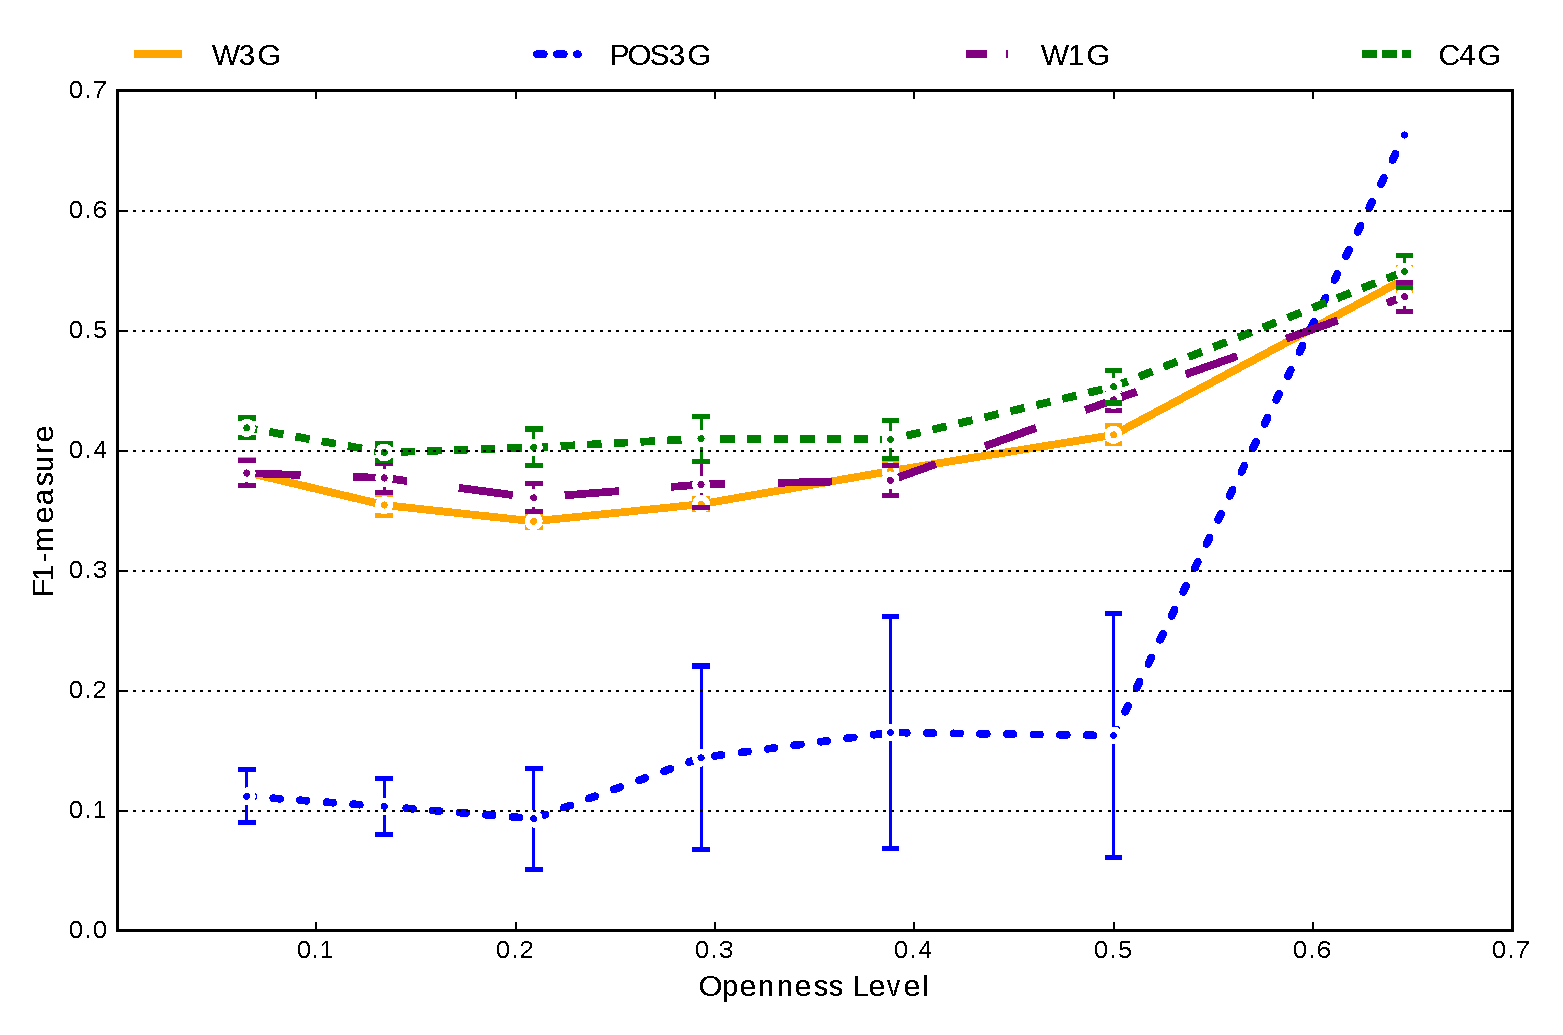
\includegraphics[scale=0.45]{Figures/OCSVME_openness_test_graph.eps}
	\caption{OCSVM performance in varying openness level.}
	\label{chap:noise:fig:OCSVME_openness_test}
\end{center}
\end{figure}

\begin{figure}[t]
\begin{center}
    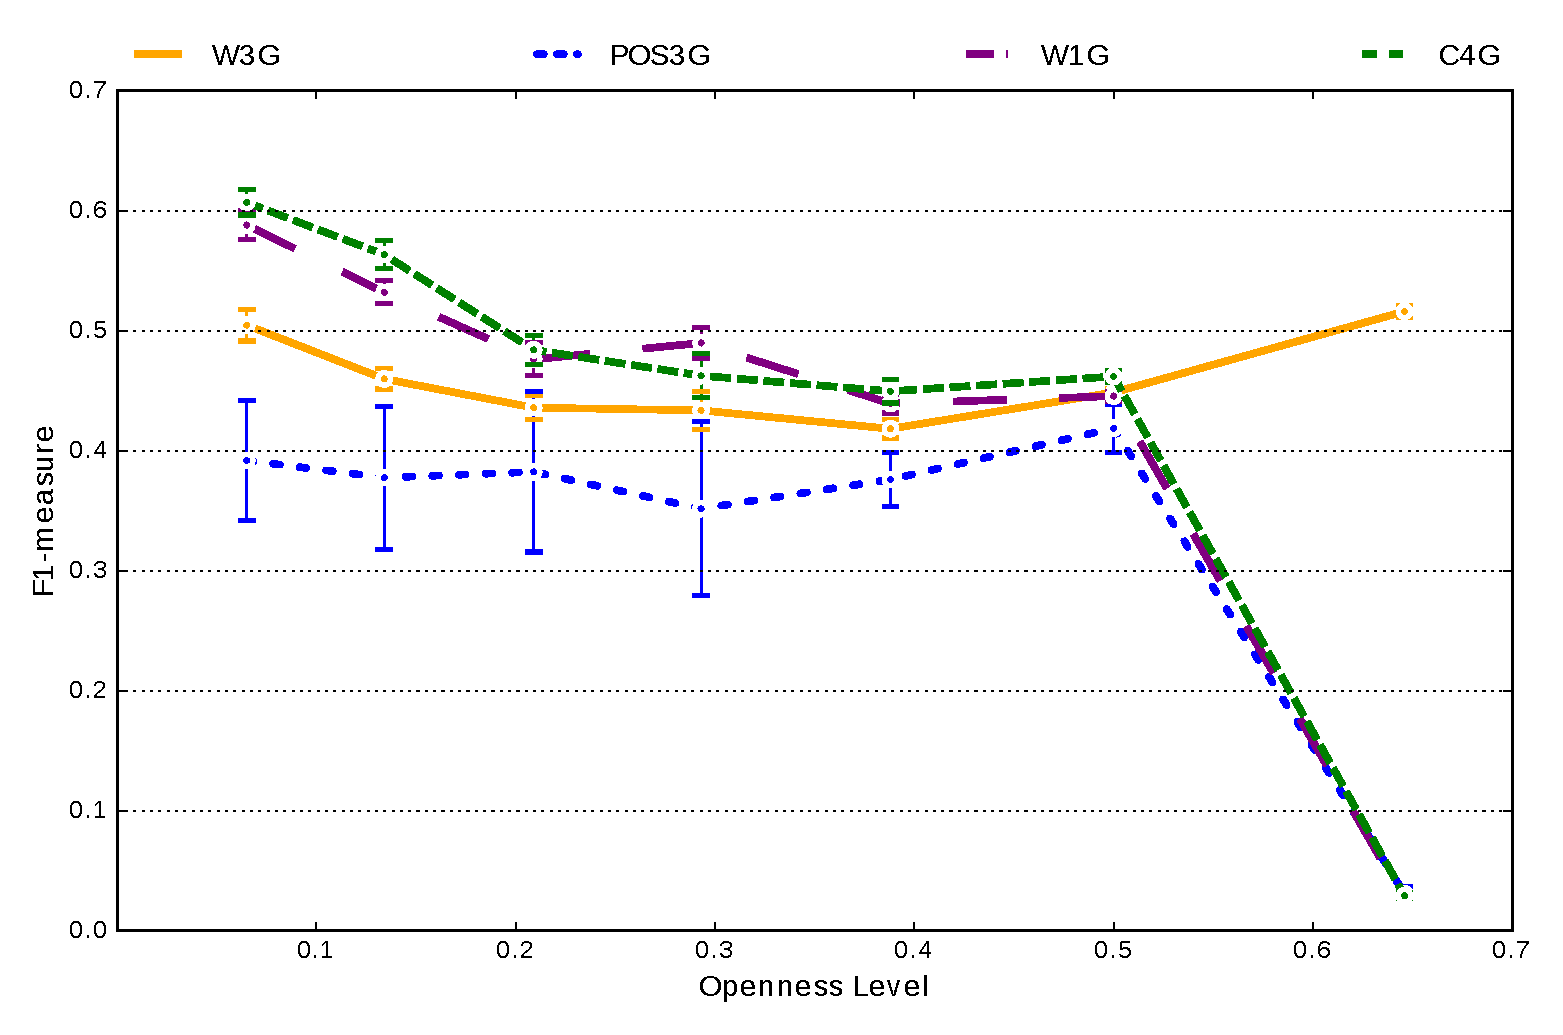
\includegraphics[scale=0.45]{Figures/RFSE_MIX_openness_test_graph.eps}
	\caption{RFSE performance in varying openness level.}
	\label{chap:noise:fig:RFSE_openness_test}
\end{center}
\end{figure}


As it was highlighted in the previous section, according to the properties of the application in which WGI is involved, precision may be more important than recall or vice-versa. In figure \ref{chap:noise:fig:RFSE_precision_focus_openness_test} the macro-precision of RFSE is depicted for W3G, W1G and C4G features. MinMax similarity is used since it increases significantly the performance of RFSE in respect with precision. As concerns text representation, W1G is the best choice when precision is at more importance than recall. On the other hand, W3G features seem to be more stable because the standard error is lower than that of the other features and also the W3G model is not affected too much when openness surpasses $0.5$ (actually it improves).

\begin{figure}[t]
\begin{center}
    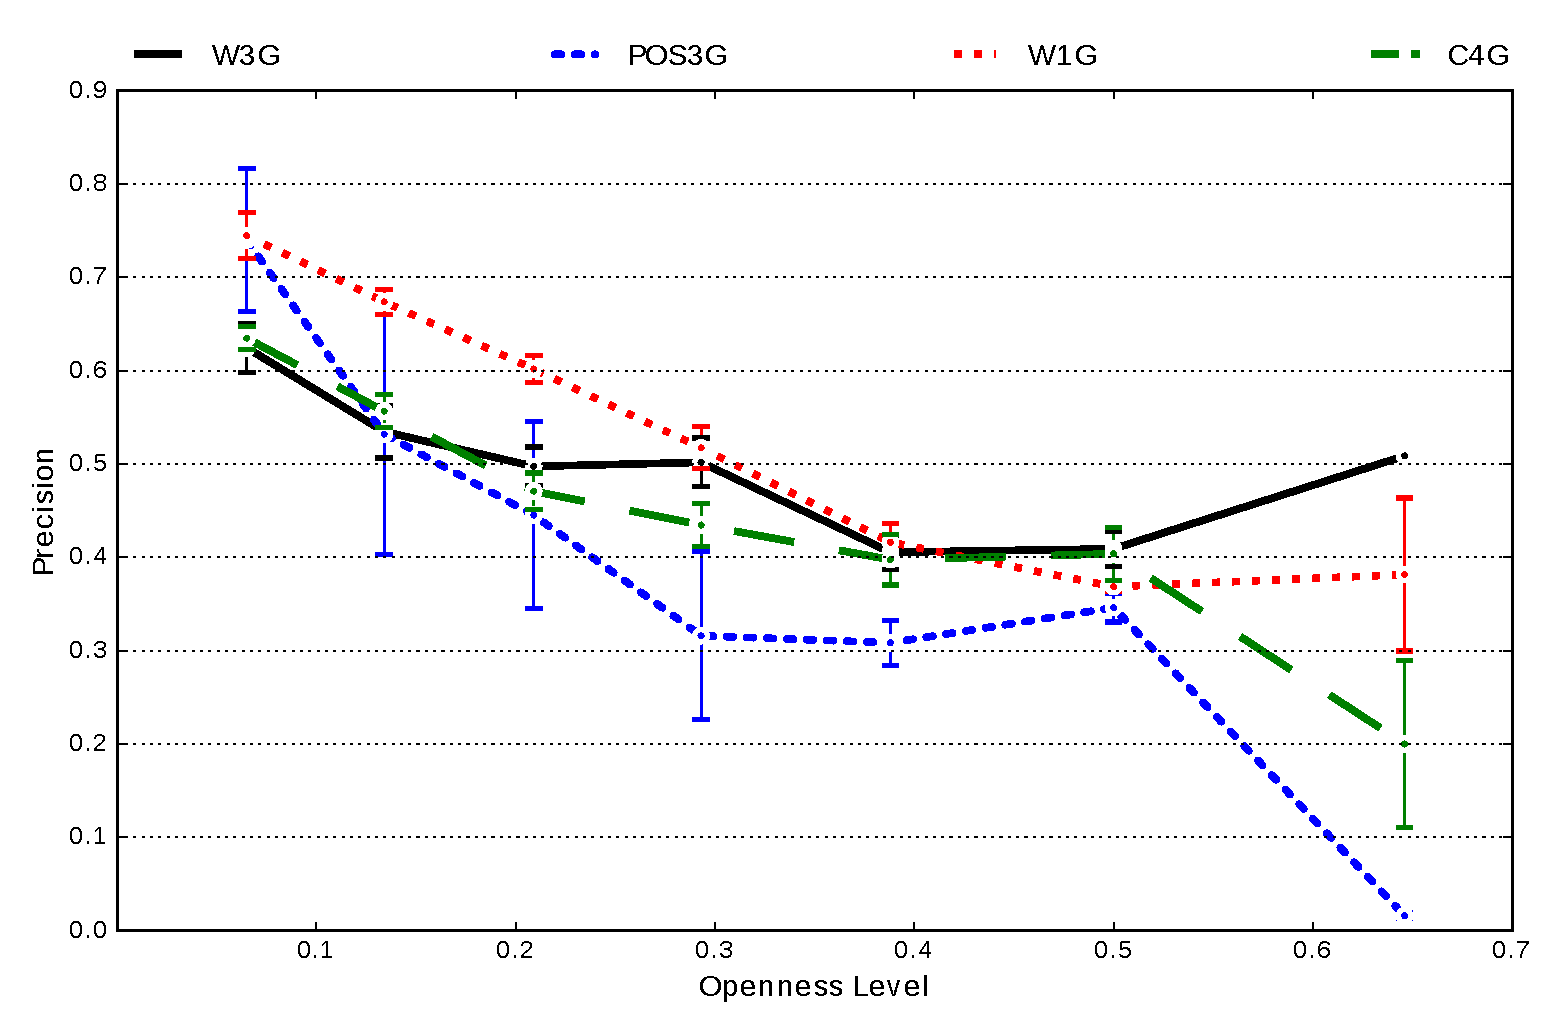
\includegraphics[scale=0.45]{Figures/RFSE_Precision_Focus_openness_test_graph.eps}
	\caption{RFSE precision in varying openness level.}
	\label{chap:noise:fig:RFSE_precision_focus_openness_test}
\end{center}
\end{figure}

In the case of C4G and W1G where the openness level is $0.646$ the standard error in both case is high. Since, this problem is only occurring in the case where the problems has been reduced to binary, it is interesting to see whether it is caused by choice of the document representation or by the choice of the similarity measure.

%In figures \ref{chap:noise:fig:RFSE_MIXvsMinMax_W3GvsC4G_openness_test} the $F_{1}$ measure performance in %the openness test of the RFSE is depicted. In all three cases we see the only with MinMax %similarity the standard error is significantly high especially in the case of $0.646$ openness %level.

Despite OCSVM's improvement when structured noise is used, it can only be competitive to RFSE on a high openness level, where all genre labels but one are considered unknown. This can be better viewed in figure \ref{chap:noise:fig:RFSE_vs_OCSVME_W1G_openness_test} where OCSVM is compared with RFSE models based on MinMax and Combo similarity measures for a varying openness level. These curves correspond to W1G features, so they are not the optimal models. However, they provide a fair comparison between examined methods. As standard error bars indicate, the performance of RFSE models with respect to the $F_{1}$ measure is significantly better than that of OCSVM while openness is less than $0.5$. Beyond that level, OCSVM is significantly better than RFSE models. It should also be noted that Combo measure helps RFSE in while openness is relatively low and MinMax seems to be a better choice when openness increases.

\begin{figure}[t]
\begin{center}
    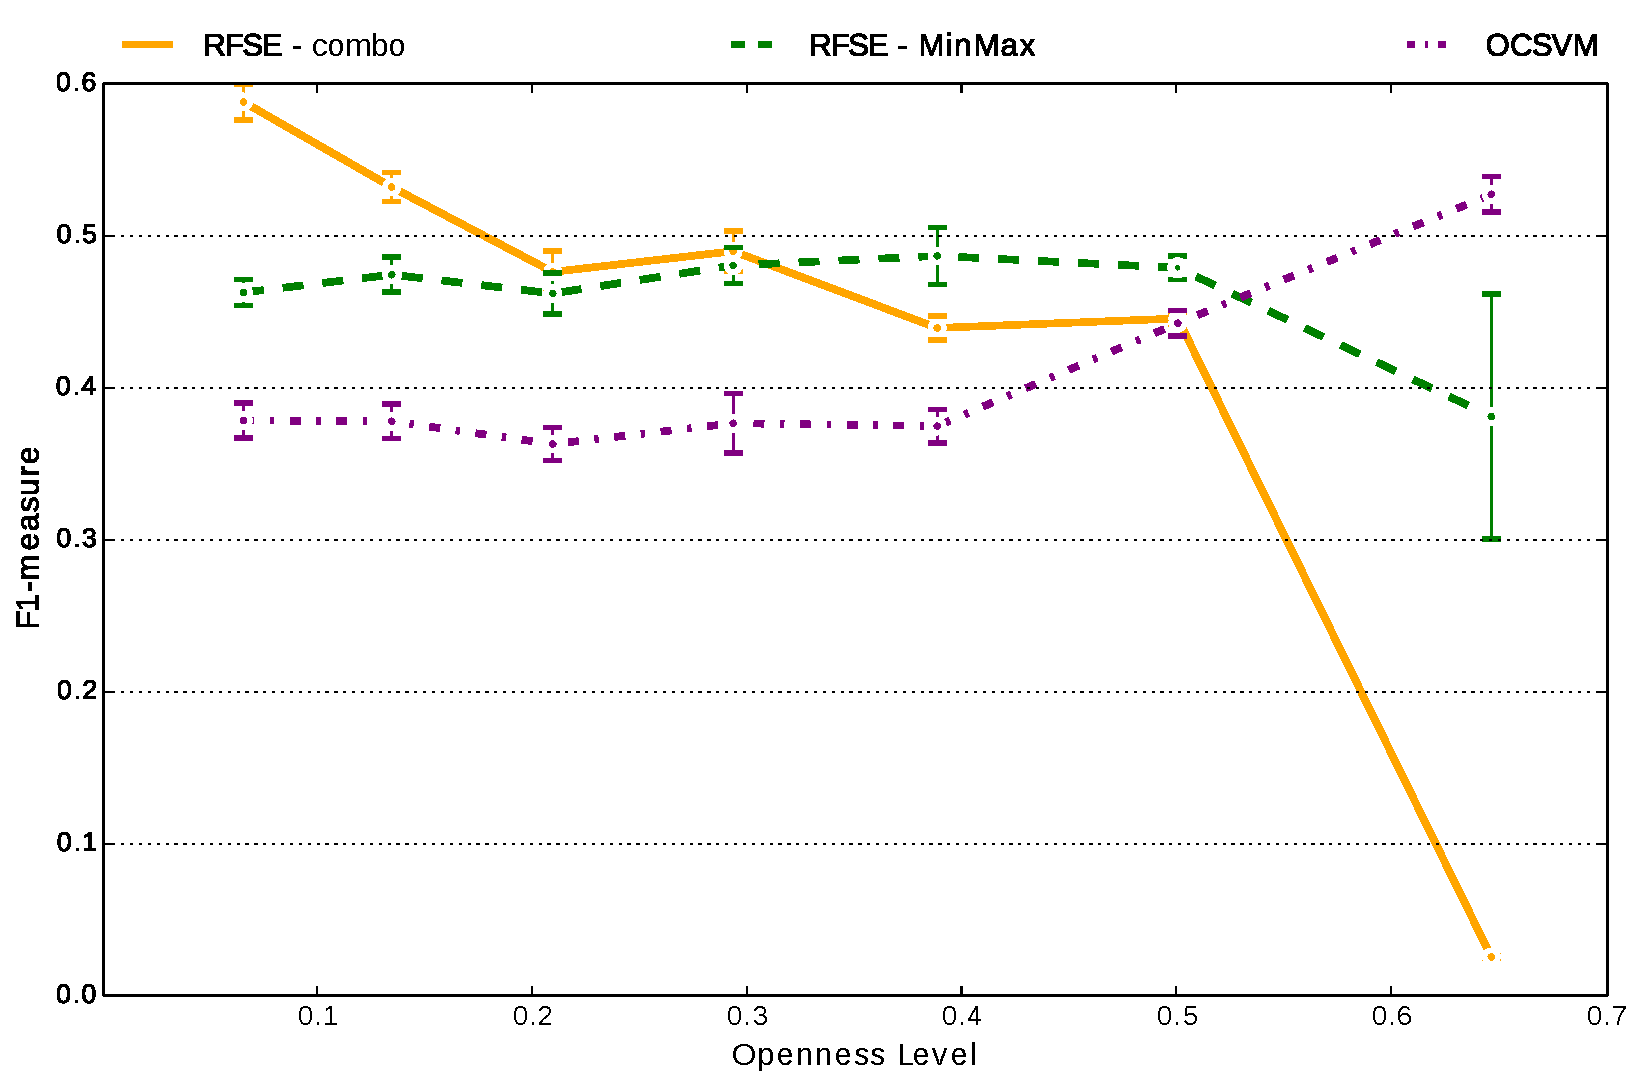
\includegraphics[scale=0.45]{Figures/RFSE_vs_OCSVME_W1G.eps}
	\caption{Comparison of OCSVM and RFSE models based on W1G features in varying Openness levels.}
	\label{chap:noise:fig:RFSE_vs_OCSVME_W1G_openness_test}
\end{center}
\end{figure}

\section{Conclusions}\label{chap:noise:sec:conclusions}

In this chapter it has been presented an experimental study on WGI focusing on open-set evaluation for this task. In contrast to vast majority of previous work in this area, the open-set scenario is adopted which is more realistic for WGI, since it is not feasible to construct a genre palette with all available genres and appropriate samples for each one of them. Moreover, we examined two open-set classification methods and several feature types and similarity measures.

The presented evaluation of open-set WGI covers two basic scenarios. The first is when noise is unstructured, i.e., information about the true genre of pages not belonging to the known genre palette is not available. The second scenario applies when noise is structured, i.e., we actually know the true genre of pages not included in the training classes. For both cases they have been used the proposed appropriate evaluation methodologies for the open-set classification, presented in chapter \ref{chap:eval_methods}.

In almost all examined cases, RFSE models outperformed the corresponding OCSVM models. This verifies previous work findings about the appropriateness of RFSE for WGI \parencite{pritsos2013open}. RFSE is able to provide effective models and additionally it is possible to manage preference on recall or precision, an application-dependent choice, by focusing on optimizing AUC or $F_1$ respectively. On the other hand, OCSVM proved to be the best-performing method in extreme cases when openness is high. Actually, the restrictions of the available corpora did not allow us to examine cases where openness approaches $1.0$. However, it seems that when openness is more than $0.5$ OCSVM outperforms RFSE.

As concerns the feature types, in most of the cases W3G and C4G provided the best results. However, the selection of text representation features is a crucial choice that affects performance and it seems to be corpus-dependent. Another crucial parameter of RFSE is the similarity measure. Among the examined measures, MinMax and its combination with cosine similarity provide the most robust results. The choice of similarity measure correlates with feature types. It seems that the combo measure is more effective than MinMax in low openness conditions.

To enhance the evaluation of WGI models in open-set conditions, we need larger corpora including multiple genre labels. New enhanced open-set WGI methods are needed and they should be evaluated using the proposed paradigm. Otherwise, using an evaluation paradigm more appropriate for closed-set tasks, the performance may be over-estimated.